\pentry{定积分\upref{DefInt},$\Gamma$ 函数\upref{Gamma}}
\subsection{结论}
\begin{equation}
{V_n} = \left\{ \begin{aligned}
&\frac{{{R^n}}}{{\left( {n/2} \right)!}}{\pi ^{\left( {n - 1} \right)/2}} &&(n = 2n-1)\\
&\frac{{{R^n}}}{{\left( {n/2} \right)!}}{\pi ^{n/2}} && (n = 2n)
\end{aligned}\right. 
= \frac{\pi ^{n/2}{R^n}}{\Gamma (1 + n/2)}
\end{equation}
 
\subsection{说明}
若定义 $n$ 维球体的表面满足方程 $\sum\limits_{i = 1}^n {x_i^2}  = R_n^2$, 其中 ${x_i}$ 为 $n$ 维直角坐标系中第 $i$ 个坐标.所有满足 $\sum\limits_{i = 1}^n {x_i^2}  \le R_n^2$ 的坐标点都定义为球内的点,且定义 $n$ 维直角坐标系中的体积为 ${V_n} = \int {\D {x_1}\D {x_2}\dots\D {x_n}} $, 积分是对所有球内的点积分.

如果这些定义看起来很抽象,不妨代入到三维空间中考虑.三维直角坐标系中, ${x_1},{x_2},{x_3}$ 分别是 $x,y,z$,  ${R_3}$ 是球的半径,球表面上任意一点都满足 ${x^2} + {y^2} + {z^2} = R_3^2$, 且球的体积分为 $\int {\D x\D y\D z} $ 是对球内部的所有点积分.
另外,若把上述定义代入到 1 维和 2, 不难发现所谓的“1 维球”和“2 维球”分别是半径为 ${R_1}$ 的线段和半径为 ${R_2}$ 的圆.
\subsection{推导}
由于正常人的空间想象力最高是 3 维,我们先由 3 维以内的球体总结出体积的递推公式,这样即使我们无法想象高维球的形状,也可以计算其体积.下面在推导前 3 个维度时,请把所有 ${x_1}{x_2}{x_3}$ 想象成 $xyz$. 
\begin{figure}[h]
\centering
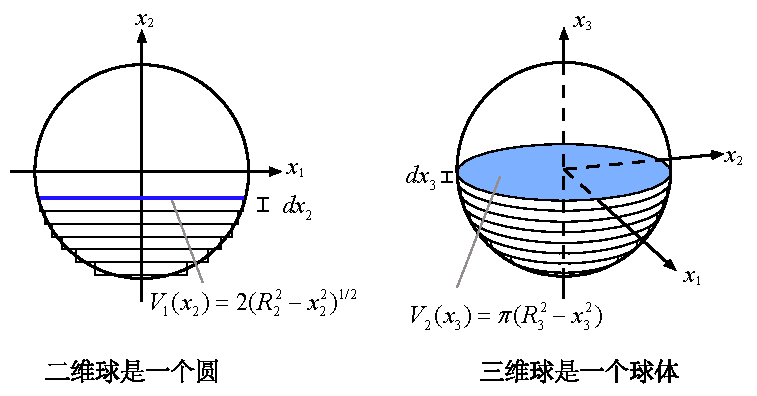
\includegraphics[width=12cm]{./figures/NSphV.pdf}
\caption{二维和三维球的体积}
\end{figure}
\subsection{ 1 维球}
这是一条线段,满足 $x_1^2 \le R_1^2$, “体积”就是线段长度
\begin{equation}\label{NDimSphV_eq1}
{V_1} = \int {\D {x_1}}  = 2{R_1}
\end{equation}
\subsection{ 2 维球}
这是一个圆,满足 $x_1^2 + x_2^2 \le R_2^2$, 在计算体积 ${V_2} = \int {d{x_1}d{x_2}} $ 时,可以先对 ${x_1}$ 积分再对 ${x_2}$ 积分
\begin{equation}\label{NDimSphV_eq2}
{V_2} = \int {\left( {\int {\D {x_1}} } \right)\D {x_2}}  = \int {{V_1}\left( {{x_2}} \right)\D {x_2}} 
\end{equation}
在几何上,这就是说把圆从沿 ${x_1}$ 轴切成许多一维球(线段),由 $x_1^2 \le R_2^2 - x_2^2$, 一维球的半径为 ${R_1}\left( {{x_2}} \right) = {(R_2^2 - x_2^2)^{1/2}}$. 代入\autoref{NDimSphV_eq1}, 得 ${x_2}$ 处切出的一维球的体积(线段的长度)为
\begin{equation}\label{NDimSphV_eq3}
{V_1}\left( {{x_2}} \right) = \int {\D {x_1}}  = 2{R_1} = 2{(R_2^2 - x_2^2)^{1/2}}
\end{equation}
再代入\autoref{NDimSphV_eq2}, 得二维求的体积为(注意 $ - {R_2} < {x_2} < {R_2}$ )
\begin{equation}\label{NDimSphV_eq4}
{V_2} = \int {{V_1}\D {x_2}}  = \int {2{{(R_2^2 - x_2^2)}^{1/2}}d{x_2}}  = \pi R_2^2
\end{equation}
\subsection{ 3 维球}
这是一个球体,满足 $x_1^2 + x_2^2 + x_3^2 \le R_3^2$, 计算体积 ${V_3} = \int {d{x_1}d{x_2}} d{x_3}$ 时,可以先对 ${x_1}{x_2}$ 积分
\begin{equation}\label{NDimSphV_eq5}
{V_3} = \int {\left( {\int {\D {x_1}\D {x_2}} } \right)\D {x_3}}  = \int {{V_2}\left( {{x_3}} \right)\D {x_3}} 
\end{equation}
在几何意义上,这是说把求沿 ${x_1}{x_2}$ 平面切成许多二维球(圆),然后把求的体积(面积)沿 ${x_3}$ 轴积分.由 $x_1^2 + x_2^2 \le R_3^2 - x_3^2$, 得 ${x_3}$ 处二维球半径为 ${R_2} = {(R_3^2 - x_3^2)^{1/2}}$. 由\autoref{NDimSphV_eq4}得体积为
\begin{equation}\label{NDimSphV_eq6}
{V_2}\left( {{x_3}} \right) = \pi R_2^2 = \pi (R_3^2 - x_3^2)
\end{equation}
代入\autoref{NDimSphV_eq5} 得三维球体积(注意 $ - {R_2} < {x_2} < {R_2}$)
\begin{equation}\label{NDimSphV_eq7}
{V_3} = \int {{V_2}\left( {{x_3}} \right)\D {x_3}}  = \int {\pi (R_3^2 - x_3^2)\D {x_3}}  = \frac{4}{3}\pi {R^3}
\end{equation}
\subsection{ $n$ 维球}
由以上两个推导,可以在代数上总结出递推的规律.把 $n$ 维球在 $n+1$ 维积分,得(可使用  Mathematica 软件计算积分,见 Mathematica 积分)%未完成:链接
\begin{gather}
{V_4} = \int_{ - R}^R {\frac{4}{3}\pi {{\left( {R_4^2 - x_4^2} \right)}^{3/2}}\D {x_4}}  = \frac{1}{2}{\pi ^2}{R^4}\\
%
{V_5} = \int_{ - R}^R {\frac{1}{2}{\pi ^2}{{\left( {R_5^2 - x_5^2} \right)}^{4/2}}\D {x_5}}  = \frac{8}{{15}}{\pi ^2}{R^5}\\
%
{V_6} = \int_{ - R}^R {\frac{8}{{15}}{\pi ^2}{{\left( {R_6^2 - x_6^2} \right)}^{5/2}}\D {x_6}}  = \frac{1}{6}{\pi ^3}{R^6}\\
%
{V_7} = \int_{ - R}^R {\frac{1}{6}{\pi ^3}{{\left( {R_7^2 - x_7^2} \right)}^{6/2}}\D {x_6}}  = \frac{{16}}{{105}}{\pi ^3}{R^7}
\end{gather}
对奇数项和偶数项分别总结规律,不难发现
\begin{equation}
{V_n} = \left\{ \begin{aligned}
&\frac{R^n}{(n/2)!} \pi ^{(n - 1)/2} &&(n= 2n - 1)\\
&\frac{R^n}{(n/2)!} \pi ^{n/2} &&(n=2n)
\end{aligned} \right.
\end{equation}
半整数的阶乘的定义\upref{Gamma} 为
\begin{equation}
\frac{n}{2}! = \frac{n}{2} \vdot \left(\frac{{n}}{2}-1\right)\dots\frac{1}{2}\sqrt{\pi}
\end{equation}
若用 $\Gamma $ 函数\upref{Gamma} 表示以上结果,就是
\begin{equation}
{V_n} = \frac{\pi ^{n/2}{R^n}}{\Gamma (1 + n/2)}
\end{equation}








